\subsection{Podnikové informační systémy}
%%%%%%%%%%%%%%%%%%%%%%%%%%%%
Pojďme se zaměřit na podniky a podnikové informační systémy (PIS), které slouží k podpoře chodu a řízení podniků. \cite{Tvrdikova2008}

Nejdříve si ujasněme co je to podnik. Následující obecnou definici ve své knize představuje Pour:
\begin{definition}
Podnik je subjekt, ve kterém dochází k přeměně zdrojů (vstupů) na statky (výstupy). \cite{Pour2015}
\end{definition}

Ten dále popisuje, že v rámci informatiky se nelze zaměřit pouze na podniky komerční, ale je nutné pojem vnímat obecněji, jako označení pro všechny typy organizací.

Podnik je možné vnímat i jako systém, uměle vytvořený fyzickou nebo právnickou osobou. 

Charakteristická pro podnik je soustava cílů, kterou určuje podnikatel. Konkretizace těchto cílů je předpokladem pro vytvoření podniku tak, aby cíle byly naplněny. \cite{Pour2015}

Jednotlivé typy podnikových informačních systému, se dají rozložit podle procesů, které mají podporovat. Hierarchické rozdělení PIS popisují různí autoři \cite{Tvrdikova2008}\cite{Vymetal2009}\cite{Basl2012}, ti systémy dělí na tři úrovně a představují příklady:

\begin{enumerate}
    \item Strategické.
    \begin{itemize}
        \item EIS -- Executive IS
    \end{itemize}
    \item Taktické.
    \begin{itemize}
        \item DSS -- Decision Support System
        \item MIS -- Management IS
    \end{itemize}
    \item Operativní.
    \begin{itemize}
        \item SCM -- Supply Chain Management
        \item CRM -- Customer Relationship Management
        \item MRP -- Material Requirements Planning
    \end{itemize}
\end{enumerate}

Na nejnižší úrovni se nachází operativní systémy sloužící k řízení základních agend a operací. Informace z této úrovně se transformují do podkladů pro taktické rozhodování. Do tohoto taktického rozhodování patří například oblasti tvorby cen, marketingu a dalších rozhodovacích procesů.

Na nejvyšší úrovni probíhají strategická rozhodování, analýzy a postupy, které se souhrnně označují pod pojmem Business Inteligence. \cite{Vymetal2009}

Komplexní systémy, které přesahují napříč všemi úrovněmi jsou označovány zkratkou ERP -- Enterprise Resource Planning.

Tato hierarchie je vidět na následujícím obrázku \ref{fig:IS_hierarchy}.

\begin{figure}[h!]
    \centering
    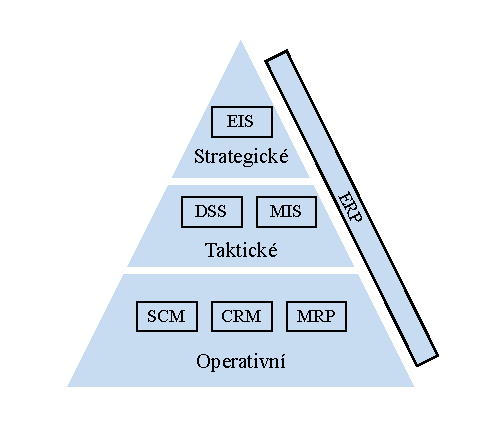
\includegraphics[width=0.6\textwidth]{assets/2_IS/IS_hierarchy.drawio.pdf}
    \caption{Hierarchie IS.}
    \label{fig:IS_hierarchy}
\end{figure}
\FloatBarrier

Nutno dodat, že toto rozdělení se mezi jednotlivými zdroji mírně liší, Bruckner \cite{Bruckner2012} systémy rozděluje až do šesti úrovní. Tyto úrovně zhruba odpovídají původním třem úrovním. Můžeme tak odvodit, že granularita rozdělení těchto systému není pevně daná.

Z této hierarchie lze odvodit, že systémy pro podporu malých podniků je vhodné začít budovat \uv{odspoda}, aby přinesly co největší užitek operativě. 

Pro účely této práce se pojďme zaměřit na CRM systémy.

